%! Author = kucera-lukas
%! Date = 4/11/22

\section{Ostatni}\label{sec:ostatni}

\subsection{Barevný motiv}\label{subsec:barevny-motiv}
Aplikace umožňuje změnu barevného motivu.
Staci kliknout na ikonku v pravem hornim rohu.
Motiv lze take prepnout klavesovou zkratkou \texttt{ctrl + k}.
Vybrany motiv se ulozi do \texttt{Window.localStorage}
\url{https://developer.mozilla.org/en-US/docs/Web/API/Window/localStorage}
a tak neni potreba motiv upravovat pri kazdem vstupu na webovou stranku.

\begin{figure}
    \centering
    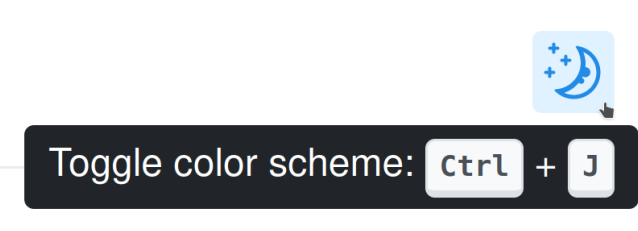
\includegraphics[scale=0.7]{assets/images/color-scheme}
    \caption{Barevny motiv}\label{fig:barevny-motiv}
\end{figure}
